\subsection{Complete input-stratified common-summary results}\label{sec:coverage}
Positive non-diagonal published demands are stratified by demand and directed free-flow shortest-path time using empirical tertiles, with ties kept in the lower bin. Within each of nine cells, lexicographically sorted OD indices at zero-based positions $\lfloor N/3\rfloor$ and $\lfloor2N/3\rfloor$ are retained. No attribution values enter selection. Endpoint differences identify total edge attribution, without identifying the same-state study/background response split. The two perturbation widths share every field of the selection protocol and differ only in the demand interval; their normalized errors are close for every query, so Table~\ref{tab:coveragefull} reports both in one table. Absolute minima, maxima, midpoints and half-ranges for both widths, and the per-position account sequences behind the segmentation of Proposition~\ref{prop:segmented}, accompany the result arrays in the code package. Figure~\ref{fig:coverageintervals} plots the complete interval set, normalized by each query's largest account magnitude; each query's common value and error follow from the tabulated range by the midpoint rule $\beta=(\phi_{\min}+\phi_{\max})/2$.
\begin{table}[pos=htbp]\centering\footnotesize\caption{Complete geometric common summaries for the 18 input-stratified queries at both widths. Normalized error is Eq.~\eqref{eq:normerror} at $\pm10\%$ and $\pm20\%$; ranges are $[\phi_{\min},\phi_{\max}]$ at $\pm20\%$ in Sioux Falls cost units; P and M mean positive and mixed signs at $\pm20\%$.}\label{tab:coveragefull}\begin{tabular}{lrrrrl}\toprule OD & System & Range ($\pm20\%$) & Norm.\ err.\ ($\pm10\%$) & Norm.\ err.\ ($\pm20\%$) & Sign\\\midrule
(4,3) & 507.2 & [429.0, 535.0] & 9.9 & 9.9 & P\\
(12,3) & 337.2 & [330.7, 340.2] & 1.4 & 1.4 & P\\
(6,1) & 2360.6 & [658.3, 2290.4] & 35.6 & 35.6 & P\\
(15,6) & 9390.2 & [415.4, 4433.5] & 45.3 & 45.3 & P\\
(6,21) & 4577.8 & [-3.4, 2349.4] & 50.1 & 50.1 & M\\
(18,14) & 3422.3 & [150.8, 1929.7] & 46.1 & 46.1 & P\\
(8,4) & 25097.5 & [1270.7, 15741.3] & 46.0 & 46.0 & P\\
(19,8) & 16939.7 & [733.2, 7266.4] & 45.0 & 45.0 & P\\
(11,6) & 6165.9 & [1236.4, 6106.4] & 39.9 & 39.9 & P\\
(16,2) & 17763.1 & [896.3, 9628.6] & 45.3 & 45.3 & P\\
(8,21) & 7605.5 & [752.6, 4214.1] & 41.1 & 41.1 & P\\
(14,8) & 17445.3 & [890.3, 7527.1] & 44.1 & 44.1 & P\\
(11,15) & 47925.5 & [17628.9, 27737.8] & 18.2 & 18.2 & P\\
(17,9) & 24040.9 & [5482.3, 18519.3] & 35.2 & 35.2 & P\\
(10,12) & 55214.5 & [9822.4, 33248.6] & 35.2 & 35.2 & P\\
(13,10) & 54411.9 & [2918.8, 31345.2] & 45.3 & 45.3 & P\\
(1,10) & 33917.2 & [2182.9, 20856.4] & 44.8 & 44.8 & P\\
(10,1) & 34264.5 & [2182.7, 21039.5] & 44.8 & 44.8 & P\\
\bottomrule\end{tabular}\end{table}

\begin{figure}[pos=htbp]\centering
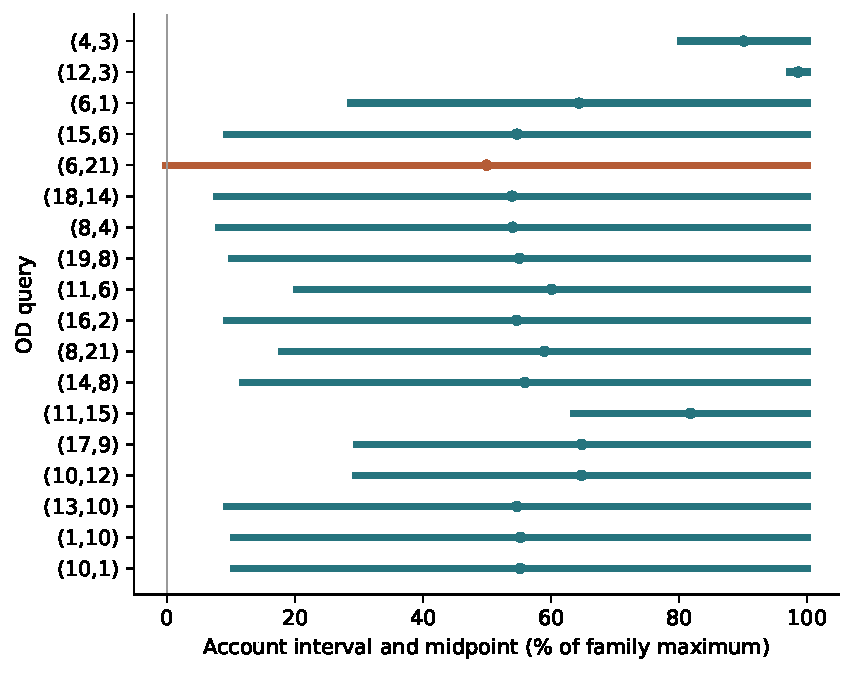
\includegraphics[width=0.88\linewidth]{../figures/fig_v108_coverage_intervals.pdf}
\caption{Geometric account intervals normalized by each query's largest
account magnitude, over all 18 input-stratified queries at $\pm20\%$
(the complete-interval companion of
Figure~\ref{fig:commonsummary}).}\label{fig:coverageintervals}
\end{figure}

\begin{table}[pos=htbp]\centering\footnotesize
\caption{Tolerance sensitivity of the delivered summaries, within
fixed projection directions (experiment C for Sioux Falls, 18 queries
per level, 36 normals with duplicate chains removed; experiment D for
Anaheim, six single-direction queries). Single: number of queries whose
whole family admits one common value at the stated tolerance;
segments: median per-direction count on Sioux Falls at load levels
$0.7/1.0/1.3$ (maximum over directions in parentheses) or per-query
range on Anaheim; compression: $1-$segments/regions, median per
direction (Sioux Falls) or per query (Anaheim).}\label{tab:tolerance}
\begin{tabular}{rrrrr}\toprule
Tolerance $\tau$ & Sioux single ($0.7/1.0/1.3$) & Sioux med.\ seg./dir. & Anaheim segments & Anaheim compression\\\midrule
$2.5\%$ & $2/1/0$ & $4.0\,(10)/4.5\,(12)/5.5\,(13)$ & $6$--$21$ & $91.5\%$\\
$5\%$ & $2/1/0$ & $3.0\,(7)/4.0\,(8)/4.5\,(10)$ & $4$--$14$ & $93.8\%$\\
$7.5\%$ & $2/1/1$ & $2.0\,(7)/3.0\,(8)/3.0\,(8)$ & $3$--$12$ & $95.5\%$\\
$10\%$ & $2/2/1$ & $2.0\,(6)/2.0\,(6)/2.5\,(7)$ & $3$--$12$ & $96.4\%$\\
\bottomrule\end{tabular}\end{table}

\paragraph{Tolerance rule and small-magnitude detail.}\label{supp:tolerance}
The primary rule is absolute: $\epsilon_j=5\%$ of the family's largest
account magnitude, so it permits errors much larger than $5\%$ of the
small accounts. A mixed rule
$|\hat a_i-a_i|\le\epsilon_{\mathrm{abs}}+\tau|a_i|$ keeps relative
control at small magnitudes; a candidate segment admits a common
representative iff $\max_{i\in I}(a_i-t_i)\le\min_{i\in I}(a_i+t_i)$
with $t_i=\epsilon_{\mathrm{abs}}+\tau|a_i|$, feasibility is inherited
by subintervals, and the same greedy returns the minimum count. On
Anaheim, at the primary rule the worst relative error at
small-magnitude positions (accounts below $10\%$ of the family
maximum) has median $0.55$ and maximum $0.94$; the mixed rule with
$\epsilon_{\mathrm{abs}}=1\%$ of the family maximum and $\tau=10\%$
lowers these to $0.28$ and $0.45$ while the median segment count rises
from 10 to 12 (per-query range 6--17), i.e.\ the compression is
essentially retained and the detail at small-magnitude positions
doubles in accuracy. Enlarging the relative part of the primary
$5\%$ absolute rule without shrinking the absolute floor
($\epsilon_{\mathrm{abs}}=5\%$, $\tau\ge5\%$) instead reduces
segment counts by merging large-magnitude runs while the
small-position error worsens --- confirming that the absolute floor,
not the relative part, controls the small-magnitude detail.

\paragraph{Load-level protocol and node-imbalance diagnostics.}
The load-level experiment solves one equilibrium per level ($0.7$,
$1.0$, $1.3$ times the published demands); with the focal query moving
alone over $\pm20\%$ under the identical geometric family and masks,
the levels $0.7$ and $1.3$ add 74 equilibrium solves. For each of the
18 columns and three levels, the imbalance vector $d_j$ of
Eq.~\eqref{eq:endpointd} has norm $\norm{d_j}_2$ rising from a median
of $1196.4$ at level $0.7$ to $4803.2$ at $1.0$ and $15763.3$ at
$1.3$ --- a $13.2$-fold increase from the light to the heavy baseline
--- while the unrestricted range $S_j$ rises from $3102.2$ to
$52766.2$. Across all 54 query--level pairs, the rank correlation
between $\norm{d_j}_2$ and the geometric-family spread is $0.99$
(Spearman; $0.99$ for $S_j$), and the realized ratio
$S_j/\norm{d_j}_2$ has median $2.53$ against the Cauchy--Schwarz bound
$\sqrt{n-2}=4.69$ of Eq.~\eqref{eq:rangebound}. The normalized
summary error, whose denominator varies by query, correlates more
moderately ($0.53$). The load levels change the realized weights,
responses and demand increments together rather than the weights alone,
so these correlations are mechanism-consistent readings of
Eq.~\eqref{eq:cutspread}, not isolated weight effects.

\subsection{Computational protocol for alternative attribution orders}\label{supp:pathrobust}
Each of the 22 alternative orders of Section~\ref{subsec:pathrobust}
changes the six study ODs one at a time (41 quadrature states per
segment, identical solver tolerance, endpoints and boundary family as
the straight-line run; canonical order, reverse order, and twenty
permutations under seed 20261031). Gates: straight-line columns
reproduce the frozen arrays to $1.7\times10^{-15}$ relative; every
order's endpoint equilibria match the straight-line endpoints to
$6.1\times10^{-9}$; the path-independent total outcome change
reproduces to $1.5\times10^{-7}$ relative. Each order's record stores
the attribution column, family range, common summary and normalized
error, sign-crossing flag, maximum profile deviation against the
straight-line accounts, and mechanism components at the fixed regions
$U_-$ (arrays in the code package). The dominant mechanism at $U_-$
coincides with the straight line's on all 22 orders for each of the
three mechanism-tracked queries.
